\section{Experimentación del algoritmo propuesto: genético con Split}
\subsection{Alcance y continuidad con las etapas anteriores}
Se tomó como algoritmo propuesto el genético con decodificación Split incluido en
el Anexo 3 del Entregable 1 del Equipo 5 \cite{equipo2026}. Esta identificación es un supuesto de
trabajo adoptado para avanzar con la experimentación: no representa un cuarto
método independiente del algoritmo genético. La comparación de cuatro métodos
debe aclarar esta coincidencia al integrar el reporte del equipo.

El cromosoma es una permutación de todos los clientes, llamada tour gigante.
Split encuentra la partición de menor distancia de ese orden en rutas factibles,
siguiendo la idea de decodificación por programación dinámica de Prins
\cite{prins2004}. La optimalidad del Split se limita a los cortes de una
permutación dada; no implica optimalidad global del CVRP. Los genéticos se han
estudiado para este problema \cite{baker2003}, pero esta implementación académica
no reproduce íntegramente esos algoritmos publicados.

\subsection{Configuración y protocolo experimental}
\begin{center}
\begin{tabular}{ll}\toprule
Elemento & Configuración fija de la etapa 1 \\\midrule
Población y generaciones & 60 individuos; 150 generaciones \\
Selección & Torneo de tamaño 3 \\
Cruce & Segmento de dos cortes, llenado lineal por orden \\
Probabilidad de cruce & 0.90 por hijo \\
Probabilidad de mutación & 0.25 por hijo \\
Mutación & Intercambio o inversión, 50\% cada una \\
Elitismo & 2 mejores individuos \\
Inicialización & Permutaciones completamente aleatorias \\
Paro & 150 generaciones, sin paro por estancamiento \\
Corridas & 3 por instancia; semillas 0, 1 y 2 \\\bottomrule
\end{tabular}
\end{center}
Se evaluaron 24 instancias (14 CMT y 10 X), para un total de 72 corridas.
Cada corrida realizó $60(150+1)=9060$ evaluaciones de individuos, incluyendo
la población inicial y la reevaluación de los élites. La reconstrucción final
se contabilizó por separado. Una generación evalúa 60 individuos; no equivale
a una iteración de ACO con 8 hormigas. No se añadió búsqueda local ni inicialización
heurística. El cruce conserva la variante de los anexos anteriores: copia un
segmento inclusivo y llena huecos de izquierda a derecha con el orden del
segundo padre; no se intercambió por otra variante circular de OX.

Las distancias se calcularon como euclidianas reales en CMT y como
$\lfloor d_{ij}+0.5\rfloor$ por arco en X. Se respetaron capacidad y cobertura
exacta. Para las instancias con duración máxima se verificó
$D_r+s|r|\leq L$, suponiendo velocidad unitaria y servicio únicamente en clientes.
El objetivo suma solo distancia, sin sumar servicio. No se impuso un límite
adicional de vehículos: los archivos no lo declaran y el algoritmo original
tampoco lo imponía. El sufijo $k$ de X se conservó como referencia del nombre.
\textbf{Si el equipo fija una flota máxima o exacta, estas corridas deben
repetirse bajo esa regla antes de compararlas.}

\clearpage
\subsection{Resultados en las 24 instancias}
Se obtuvieron soluciones factibles en las 72 corridas. La validación volvió a
calcular distancia, carga, duración y cobertura a partir de las rutas guardadas.
La tabla presenta la media, desviación estándar muestral, mejor distancia,
tiempo medio, vehículos medios y generación media de obtención del mejor valor.

\begin{center}\small
\setlength{\tabcolsep}{4pt}
\begin{tabular}{lrrrrrrr}\toprule
Instancia & $n$ & $\bar Z$ & $s_Z$ & $Z_{\min}$ & $\bar t$ (s) & $\bar k$ & $\bar g^*$ \\\midrule
CMT1 & 50 & 651.33 & 25.67 & 630.61 & 0.805 & 6.33 & 145.3 \\
CMT2 & 75 & 1167.47 & 12.41 & 1154.31 & 1.103 & 11.33 & 144.3 \\
CMT3 & 100 & 1495.49 & 88.68 & 1438.59 & 2.651 & 9.00 & 149.3 \\
CMT4 & 150 & 2427.68 & 56.71 & 2376.62 & 3.204 & 14.33 & 148.7 \\
CMT5 & 199 & 3444.23 & 112.57 & 3316.51 & 6.722 & 21.33 & 149.7 \\
CMT6 & 50 & 709.33 & 20.67 & 687.72 & 1.335 & 7.00 & 148.7 \\
CMT7 & 75 & 1330.65 & 46.59 & 1302.34 & 1.248 & 15.67 & 148.3 \\
CMT8 & 100 & 1612.29 & 110.01 & 1494.19 & 2.459 & 14.67 & 148.7 \\
CMT9 & 150 & 2782.51 & 16.69 & 2763.54 & 4.202 & 25.33 & 147.0 \\
CMT10 & 199 & 3734.40 & 125.67 & 3597.15 & 6.446 & 34.00 & 149.7 \\
CMT11 & 120 & 2544.09 & 73.34 & 2470.53 & 4.052 & 9.00 & 149.0 \\
CMT12 & 100 & 1636.03 & 77.52 & 1552.70 & 2.025 & 11.00 & 149.3 \\
CMT13 & 120 & 2823.62 & 32.62 & 2786.15 & 4.466 & 15.67 & 148.3 \\
CMT14 & 100 & 1541.51 & 67.71 & 1463.44 & 2.252 & 13.33 & 149.3 \\
X-n280-k17 & 279 & 94190.67 & 2611.60 & 91280.00 & 11.852 & 20.00 & 148.7 \\
X-n303-k21 & 302 & 70054.67 & 1839.68 & 68858.00 & 10.416 & 26.67 & 149.7 \\
X-n308-k13 & 307 & 91959.00 & 1332.85 & 90467.00 & 16.301 & 16.00 & 149.0 \\
X-n327-k20 & 326 & 92945.67 & 583.11 & 92397.00 & 12.152 & 26.33 & 148.7 \\
X-n336-k84 & 335 & 207330.67 & 723.45 & 206509.00 & 3.987 & 98.33 & 149.0 \\
X-n401-k29 & 400 & 145088.00 & 4345.30 & 140354.00 & 13.777 & 31.67 & 149.7 \\
X-n411-k19 & 410 & 92743.00 & 1817.90 & 90649.00 & 23.037 & 24.33 & 149.0 \\
X-n429-k61 & 428 & 157489.67 & 2560.32 & 155479.00 & 9.366 & 76.67 & 150.0 \\
X-n449-k29 & 448 & 167432.00 & 1883.63 & 166219.00 & 16.620 & 34.00 & 149.7 \\
X-n459-k26 & 458 & 93074.00 & 606.97 & 92627.00 & 20.586 & 35.00 & 148.3 \\
\bottomrule\end{tabular}
\end{center}
\noindent $n$: clientes, sin depósito; $\bar g^*$: generación del último descenso
estricto mayor que $10^{-8}$ en el mejor valor. Todas las corridas terminaron
en la generación 150. $\bar g^*$ no es el número total de generaciones ejecutadas.

El tiempo se midió con \texttt{perf\_counter}, en un proceso secuencial, incluyendo
inicialización de población, evolución y reconstrucción final. Se excluyeron
lectura, preparación de matriz, validación, escritura de archivos y figuras.
El total observado de tiempo de algoritmo fue 543.20 s; las corridas
oscilaron entre 0.780 y 23.392 s. Estos tiempos corresponden al entorno de
ejecución descrito en \texttt{metadatos.json}; una comparación de velocidad con
otros métodos requiere ejecutarlos en la misma máquina y con igual alcance
del cronómetro.

La reducción media frente al mejor individuo inicial fue de 43.77\%,
calculada sobre las 72 corridas. El coeficiente de variación por instancia
osciló entre 0.35\% y 6.82\%. Con solo tres repeticiones, estas
medidas son descriptivas y no demuestran superioridad estadística.

\clearpage
\subsection{Comparación con referencias de la literatura}
Se consultó la tabla de CVRPLIB \cite{cvrplib}, que reúne casos clásicos CMT y
la familia X de Uchoa y colaboradores \cite{uchoa2017}. Los valores se guardaron
con fuente y fecha de consulta. La diferencia relativa se calculó como:
\[
 \Delta_{\mathrm{ref}}(\%)=100\frac{Z-Z_{\mathrm{ref}}}{Z_{\mathrm{ref}}}.
\]
Se reporta como \emph{diferencia con referencia publicada}; no sustituye el
GAP respecto al modelo matemático del equipo. La columna ``Ópt. pub.'' reproduce
la clasificación de la fuente y no certifica optimalidad de nuestras corridas.
La comparación debe conservar convenciones equivalentes de distancia y flota.

\begin{center}\small
\begin{tabular}{lrrrr}\toprule
Instancia & $Z_{\mathrm{ref}}$ & Ópt. pub. & $\Delta_{\mathrm{media}}$ (\%) & $\Delta_{\mathrm{mejor}}$ (\%) \\\midrule
CMT1 & 524.61 & Sí & 24.15 & 20.20 \\
CMT2 & 835.26 & Sí & 39.77 & 38.20 \\
CMT3 & 826.14 & Sí & 81.02 & 74.13 \\
CMT4 & 1028.42 & Sí & 136.06 & 131.09 \\
CMT5 & 1291.29 & Sí & 166.73 & 156.84 \\
CMT6 & 555.43 & Sí & 27.71 & 23.82 \\
CMT7 & 909.68 & Sí & 46.28 & 43.16 \\
CMT8 & 865.94 & Sí & 86.19 & 72.55 \\
CMT9 & 1162.55 & Sí & 139.35 & 137.71 \\
CMT10 & 1395.85 & Sí & 167.54 & 157.70 \\
CMT11 & 1042.12 & Sí & 144.13 & 137.07 \\
CMT12 & 819.56 & Sí & 99.62 & 89.46 \\
CMT13 & 1541.14 & Sí & 83.22 & 80.78 \\
CMT14 & 866.37 & Sí & 77.93 & 68.92 \\
X-n280-k17 & 33503.00 & No & 181.14 & 172.45 \\
X-n303-k21 & 21736.00 & No & 222.30 & 216.79 \\
X-n308-k13 & 25859.00 & No & 255.62 & 249.85 \\
X-n327-k20 & 27532.00 & No & 237.59 & 235.60 \\
X-n336-k84 & 139111.00 & No & 49.04 & 48.45 \\
X-n401-k29 & 66154.00 & No & 119.32 & 112.16 \\
X-n411-k19 & 19712.00 & No & 370.49 & 359.87 \\
X-n429-k61 & 65449.00 & No & 140.63 & 137.56 \\
X-n449-k29 & 55233.00 & No & 203.14 & 200.94 \\
X-n459-k26 & 24139.00 & No & 285.58 & 283.72 \\
\bottomrule\end{tabular}
\end{center}
La diferencia media no ponderada entre instancias fue de 94.26\% en CMT y
206.48\% en X. La menor diferencia media se observó en CMT1
(24.15\%) y la mayor en X-n411-k19 (370.49\%). Los resultados muestran
que la configuración original produce soluciones factibles, pero su calidad
queda lejos de las referencias en buena parte de estas instancias. Se debe
reportar esta limitación, sin atribuirle al algoritmo un desempeño que no obtuvo.
Como detalle de trazabilidad, el archivo suministrado CMT11 tiene comentario
1042.11; para esta tabla se usó 1042.12, valor consultado en CVRPLIB.

\clearpage
\subsection{Convergencia y tiempo de cómputo}
\begin{figure}[H]\centering
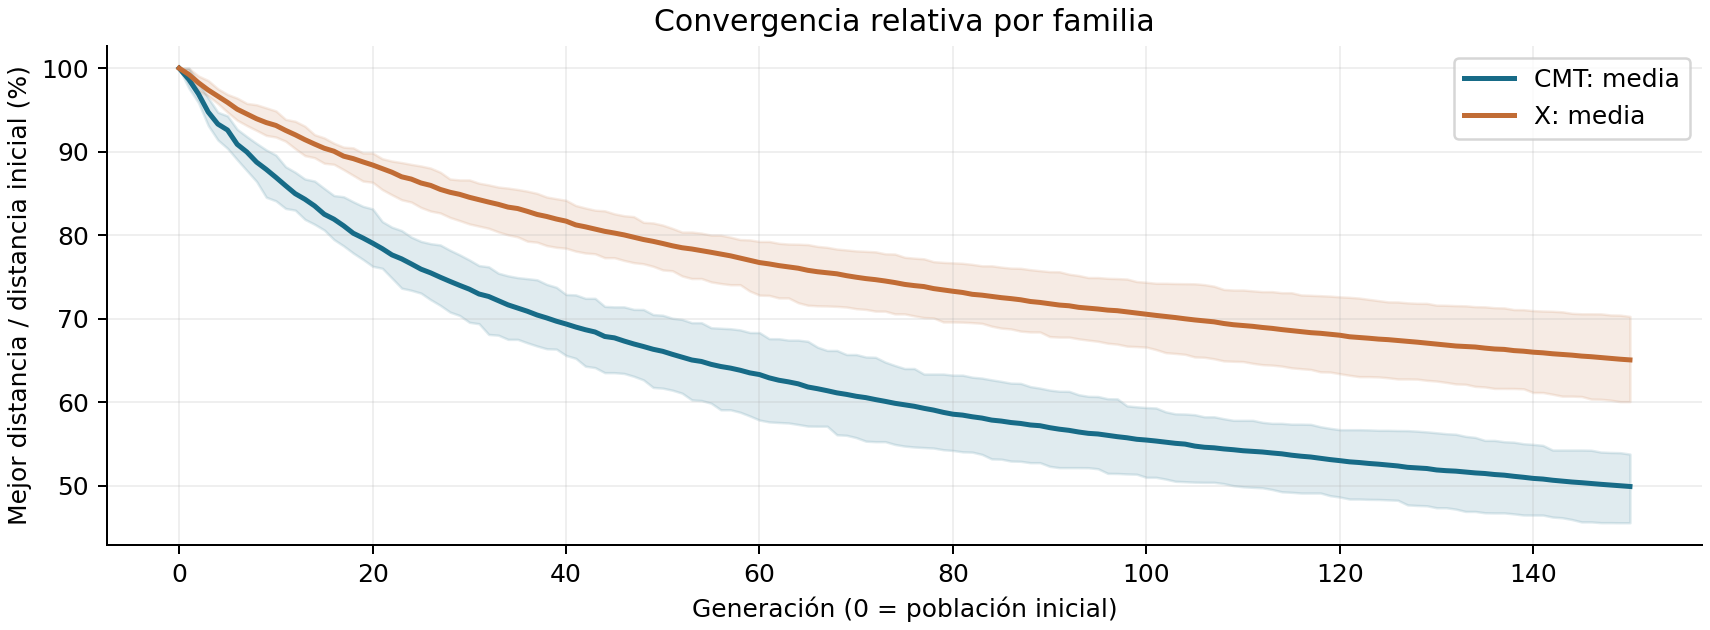
\includegraphics[width=\linewidth]{graficas/propuesto/convergencia.png}
\caption{Mejor distancia normalizada por la mejor distancia inicial de cada
corrida. Líneas: media de 42 corridas CMT y 30 X; bandas: percentiles 25 y 75,
no intervalos de confianza. Menor porcentaje indica mayor reducción relativa.}
\end{figure}
El elitismo conserva los mejores individuos y explica la trayectoria no
creciente del mejor costo. La normalización permite describir avance relativo
sin mezclar distancias absolutas de escalas distintas; no permite comparar
dificultad ni calidad final entre familias por sí sola.
\begin{figure}[H]\centering
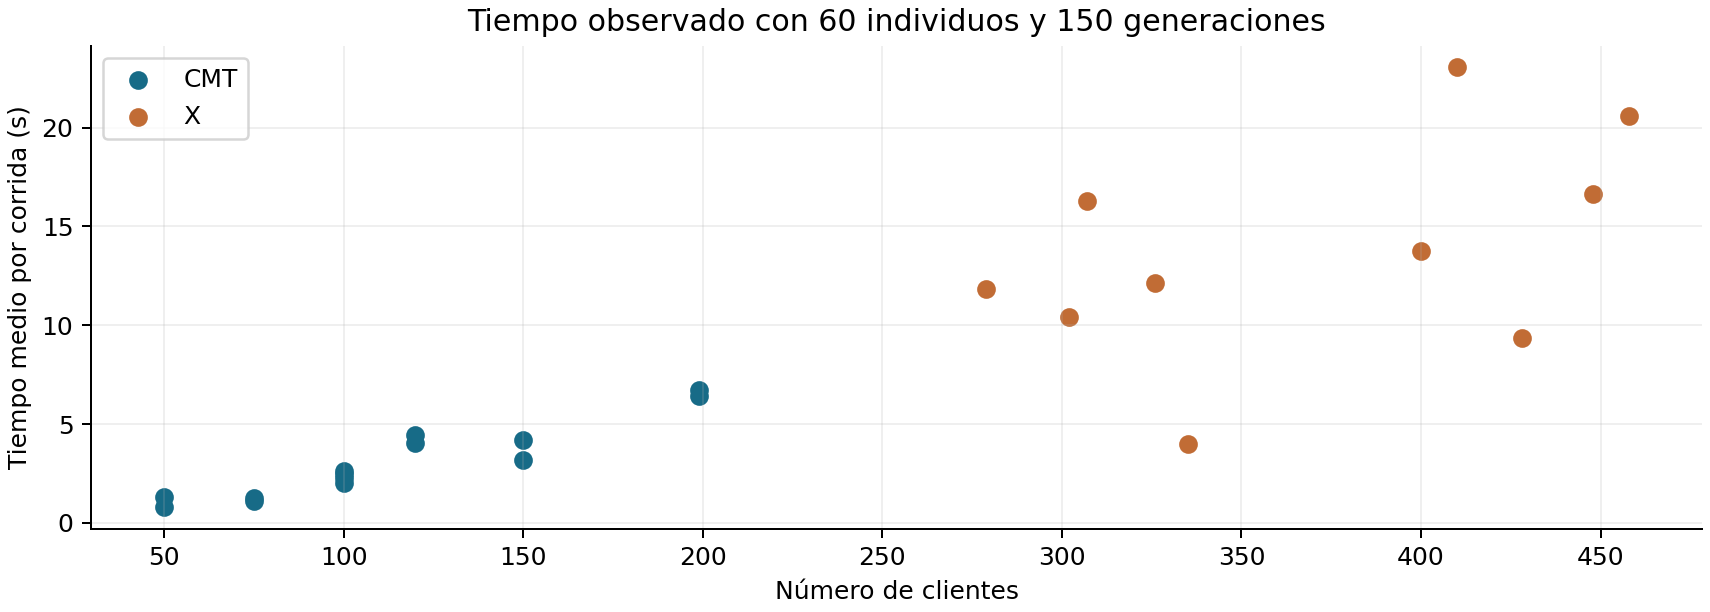
\includegraphics[width=\linewidth]{graficas/propuesto/tiempos.png}
\caption{Tiempo medio por instancia con una configuración fija. El número de
clientes no es el único factor: capacidad y duración cambian cuántos tramos
factibles evalúa Split.}
\end{figure}

\clearpage
\subsection{Ejemplo de solución y conclusiones de esta parte}
\begin{figure}[H]\centering
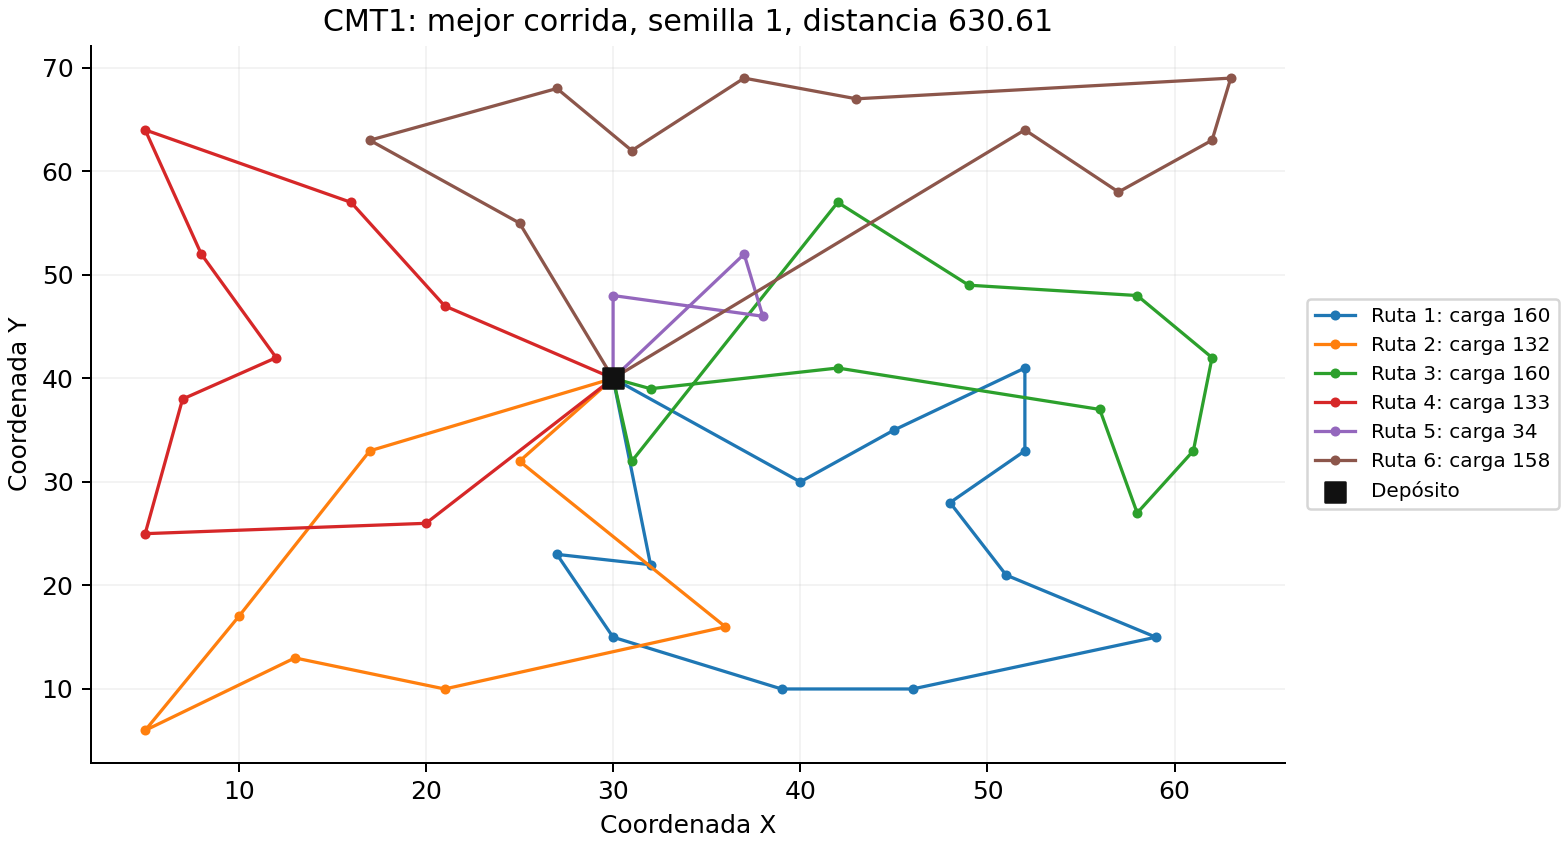
\includegraphics[width=0.98\linewidth]{graficas/propuesto/rutas_CMT1.png}
\caption{Mejor solución observada en CMT1. Cada color es una ruta que sale
y regresa al depósito; las cargas se verificaron contra la capacidad 160.}
\end{figure}
El algoritmo de la etapa 1 pudo adaptarse a las 24 instancias y generó soluciones
factibles en todas las corridas bajo las reglas declaradas. Sin embargo, el buen
resultado previo en un caso de 10 clientes no se trasladó automáticamente a
problemas de entre 50 y 458 clientes. La diferencia con las referencias muestra
que la factibilidad y el bajo tiempo no bastan para concluir que las soluciones
son competitivas.

Una explicación posible es el presupuesto fijo de población y generaciones,
combinado con inicialización aleatoria y ausencia de búsqueda local. Esta es una
interpretación del diseño, no una prueba causal: habría que experimentar con
esas variantes para comprobarla. En esta parte se conservaron los parámetros
anteriores para medir una línea base; no se hizo un estudio de sensibilidad
nuevo y por tanto no se identificaron niveles ``óptimos'' para instancias grandes.

El estudio factorial de cruce, mutación y selección corresponde a la parte del
genético asignada al otro integrante. Esta línea base puede incorporarse a esa
comparación, pero no debe contarse como un algoritmo independiente si ambos
usan el mismo método. La superioridad entre modelo, GA, ACO y otro método
distinto sigue pendiente de integrar los resultados del equipo con reglas iguales.

\clearpage
\subsection{Reproducibilidad e integración con el equipo}
Los resultados individuales se entregan en \texttt{corridas.csv}; el resumen
en \texttt{resumen.csv}; las rutas, semillas, historias y validaciones en
\texttt{detalle\_corridas.json}. Los metadatos incluyen versiones, plataforma,
configuración y huellas SHA-256 de datos y código. Las figuras se generan desde
estos resultados, sin repetir la optimización.

Desde la raíz del repositorio:
\begin{verbatim}
python -m algoritmos.propuesto.ejecutar
python -m algoritmos.propuesto.generar_reporte
python -m unittest discover -s tests -v
\end{verbatim}
El algoritmo requiere Python 3.10 o posterior y solo biblioteca estándar.
Las figuras requieren NumPy y Matplotlib. Con versiones distintas de Python,
los resultados de los operadores aleatorios pueden variar aun con igual semilla.
Los archivos entregados conservan las ejecuciones aquí descritas.

Antes de juntar tablas se deben confirmar la flota permitida, las distancias y
la duración. Si ACO ya se ejecutó con otra convención, no basta con cambiar el
nombre de la columna: es necesario recalcular o repetir la optimización según
el cambio. Para el GAP con el modelo, se requiere su objetivo y estado del solver:
\[
 \operatorname{GAP}_{\mathrm{modelo}}(\%)=
 100\frac{Z_{\mathrm{propuesto}}-Z^*_{\mathrm{modelo}}}{Z^*_{\mathrm{modelo}}},
\]
solo cuando el modelo certifica optimalidad bajo las mismas reglas. Con una
solución factible sin prueba de optimalidad, se reporta diferencia con el
incumbente; con una cota inferior válida se informa una brecha respecto a esa
cota. No se fabricaron objetivos, cotas ni estados del modelo que no se recibieron.

La validación de Split se contrastó con enumeración completa de particiones
de 120 tours pequeños en cuatro regímenes de restricciones (480 comparaciones).
Además se verificaron los operadores, reproducibilidad con semilla, elitismo
y lectura de los 24 archivos. Esto comprueba el comportamiento del código en
esos casos; no demuestra optimalidad global en las instancias experimentales.
